% !TeX root = main.tex


\begin{savequote}[70mm]
,,''
\qauthor{}
\end{savequote}


\chapter{Aplikacje i~testy}
\label{chap:aplikacje}

\section{Automatyczna kalibracja odometrii i~żyroskopu}

Proces kalibracji odometrii oraz pomiarów uzyskiwanych z~żyroskopu został
przestawiony w~rozdziale~\ref{chap:software}. W~celu jego ułatwienia 
i~zautomatyzowania stworzona została aplikacja przeprowadzająca dwuetapową
kalibrację -- najpierw wyliczająca poprawki dla współczynników kątowych
żyroskopu i~odometrii, a~następnie licząca poprawkę dla składnika liniowego
odometrii. Aby poprawnie przeprowadzić cały proces wymagana jest pusta
przestrzeń o~powierzchni ok. 2x2m, oraz płaska powierzchnia na jednym z~końców
(np. ściana).

\subsection{Wyznaczanie odległości i~kąta obrotu względem ściany}

W celu wyznaczenia faktycznej wartości obrotu wykonanego przez robota oraz
określenia pokonanej odległości, wymagana jest obecność sensora zwracającego
odczyty laserowe (w~przypadku robota Elektron możliwe jest wykorzystanie
zarówno skanera SICK jak i~sensora Kinect z~dodatkowym komponentem
zamieniającym pomiary z~chmury punktów na symulację odczytu laserowego). Na
podstawie punktów zwracanych przez sensor ustawiony na przeciwko ściany
wyliczana jest orientacja robota względem niej, a~także odległość.

\subsubsection{Orientacja}

Dane odczytane z~lasera mają postać zbioru punktów we współrzędnych biegunowych.
Pierwszym krokiem jest ich przeliczenie na współrzędne kartezjańskie w~układzie
związanym ze środkiem sensora. Po takim przeliczeniu, wykorzystując metodę
najmniejszych kwadratów, wyliczane są parametry prostej przechodzącej możliwie
blisko danych punktów. Współczynnik kierunkowy tej prostej określa jednocześnie
orientację robota względem ściany.

Mając dane punkty w~postaci $(x_i, y_i)$, gdzie $i=1\ldots n$, oraz przyjmując
oznaczenia:

\[
S_x = \sum_{i=1}^n x_i \mathsp
S_y = \sum_{i=1}^n y_i \mathsp
S_{xx} = \sum_{i=1}^n x_i^2 \mathsp
S_{xy} = \sum_{i=1}^n x_i \cdot y_i \mathsp
%S_{yy} = \sum_{i=1}^n y_i^2 \mathsp
\Delta = n \cdot S_{xx} - S_x^2
\]

Współczynniki prostej o~równaniu $y=a\cdot x+b$ wyznaczane są przez wzory:

\[
a~= \frac{n \cdot S_{xy} - S_x \cdot S_y}{\Delta} \mathsp
b = \frac{S_{xx} \cdot S_y - S_x \cdot S_{xy}}{\Delta}
\]

Skąd orientację robota względem ściany (wyznaczonej prostej) uzyskujemy ze
wzoru:

\[
\phi=atan(a)
\]

\subsubsection{Odległość}

Wykorzystując już punkty we współrzędnych kartezjańskich, odległość od ściany
wyliczana jest jako średnia z~wartości $y$ wszystkich punktów.

\subsection{Właściwy proces kalibracji}

Przed rozpoczęciem kalibracji robot powinien zostać ustawiony na wprost ściany,
w~odległości ok. 50cm od niej. Pierwszą czynnością po uruchomieniu zadania jest
wyznaczenie składowej stałej pomiarów z~żyroskopu, po czym następują trzy
pełne obroty robota z~różnymi prędkościami (fakt wykonania pełnego obrotu
wyznaczany jest na podstawie odczytów z~odometrii). Po wykonaniu każdego obrotu
wyliczana jest faktyczna jego wartość (na podstawie porównania orientacji
względem ściany zmierzonej przed i~po wykonaniu obrotu), a~razem z~nią
zapamiętywane są wartości obrotu odczytane z~odometrii i~żyroskopu. Pomiędzy
kolejnymi pomiarami robot jest pozycjonowany powtórnie na wprost ściany 
(z~pewną, niewielką tolerancją) wykorzystując pomiary laserowe. Po wykonaniu
wszystkich obrotów wyliczane są błędy wskazań odometrii i~żyroskopu (stosunek
wartości odczytanej do zmierzonej laserem), a~z nich wyliczana jest średnia
wartość poprawki, którą należy wprowadzić do współczynników obrotowych obu
badanych czujników.

Po wykonaniu kalibracji obrotów robot powtórnie ustawia się na wprost ściany, 
a~następnie odjeżdża od niej na odległość ok. 2 metrów. Następnie przejeżdża 1.5
metra do przodu, a~po przejechaniu tego dystansu wyliczana jest poprawka
współczynnika liniowego odometrii (stosunek przejechanej odległości wyliczonej
przez odometrię do odległości uzyskanej z~pomiarów laserowych). Ostateczna
wartość poprawki wyliczana jest jako średnia z~trzech takich przejazdów 
z~różnymi prędkościami. Uzyskane w~tym procesie wartości współczynników należy
pomnożyć przez współczynniki już ustawione w~sterownikach robota.



\section{Prosta, losowa eksploracja}

Kolejną aplikacją, która powstała w~celu przetestowania poprawnego działania
sensorów oraz sterownika silników była losowa eksploracja terenu. Podczas
ruchu wyznaczana jest minimalna odległość do przeszkód w~dwóch strefach
-- po lewej oraz prawej stronie. Jeśli wokół robota nie ma przeszkód bliżej,
niż ustalona odległość minimalna, to porusza się on na wprost. W~przeciwnym
wypadku prędkość kątowa jest proporcjonalna do różnicy odległości przeszkód
po lewej i~prawej stronie (o kierunku takim, aby dążyć do wyrównania odległości
po obu stronach), a~prędkość liniowa proporcjonalna jest do średniej odległości
przeszkód po obu stronach.

Zadanie spełnia swoją podstawową rolę -- pozwala na przetestowanie różnych
zestawów sensorycznych (skanera laserowego, Kinecta) oraz zweryfikować
poprawność działania układu zarządzającego pracą silników. Niestety, ze względu
na bardzo prosty algorytm zastosowany do omijania przeszkód, zdarzają się sytuacje
blokady robota w~narożnikach pomieszczeń (średnia odległość od przeszkód po
obu stronach jest taka sama, więc robot nie skręca, a~ściany są na tyle blisko,
że prędkość liniowa została wyzerowana). Innym pojawiającym się problemem
jest wjeżdżanie w~przeszkody podczas zakręcania przy korzystaniu z~sensorów
o~dużej minimalnej odległości działania i~wąskim polu widzenia. Spowodowane jest
to brakiem jakiejkolwiek pamięci co do przeszkód (np. małej lokalnej mapy zajętości),
przez co jeśli robot stoi obok ściany (której nie wykrywa czujnikami, bo nie jest
w~ich polu widzenia) i~odwróci się w~jej stronę, to może na nią wjechać (czujniki
nie wykryją przeszkody, gdyż znajduje się ona zbyt blisko).



%\section{Budowa mapy}



\section{Dojazd do wyznaczonego celu z~omijaniem przeszkód}

Ostatnią, a~zarazem kluczową aplikacją stworzoną w~ramach tej pracy jest
pełny system nawigacji (o strukturze opisanej w~poprzednich rozdziałach)
przygotowany do możliwie maksymalnego wykorzystania wszystkich dostępnych
elementów (tj. układów sensorycznych, systemów lokalizacji). Eksperymenty
przeprowadzane były w~laboratorium robotyki i~jego okolicach, a~więc w~pomieszczeniach
o~charakterze biurowo-warsztatowym, z~wieloma obiektami przenoszonymi z~miejsca
na miejsce. Szczególnie często na korytarzu zmieniała się konfiguracja przeszkód
-- przestawiane krzesła, drzwi otwierane czasami częściowo, czasami całkowicie,
a~także przechodzący ludzie. Zgodnie z~założeniami zadania, robot miał poradzić
sobie w~takim środowisku i~dążyć do osiągnięcia zadanego celu.

\subsection{Scenariusz pracy}

Scenariusz działań podczas korzystania z~tej aplikacji jest dość prosty -- początkowo,
po uruchomieniu robota i~wszystkich niezbędnych modułów opisanych wcześniej, należy
wskazać jego przybliżoną pozycję i~orientację na mapie. Następnym krokiem jest
wskazanie punktu docelowego, który robot ma osiągnąć. W~zależności od jego osiągalności,
a~w~zasadzie tego, czy planer globalny będzie w~stanie wyznaczyć prawidłowy plan
czy nie, podejmowane są różne akcje. Jeśli plan nie zostanie odnaleziony, to wyświetlany
jest odpowiedni komunikat oraz emitowany dźwięk oznaczający niepowodzenie wykonania
zadania. Jeśli ścieżka zostanie wyznaczona, emitowany jest dźwięk akceptacji celu
i~rozpoczyna się wykonanie trajektorii, segment po segmencie. Podczas jazdy może się
okazać, że wyznaczona ścieżka jest niemożliwa do wykonania (np. zostały zamknięte
drzwi, przez które wiodła trajektoria), robot się zatrzymuje i~uruchamiany jest
ponownie planer globalny (z dodatkową wiedzą o~stanie przeszkód w~okolicy robota).
Po dojechaniu do wyznaczonego celu (z pewną, określaną z~góry dokładnością zarówno
co do położenia jak i~orientacji) robot zatrzymuje się i~emitowana jest informacja
o~poprawnym wykonaniu zadania.

\subsection{Obsługa sytuacji wyjątkowych}

Odrębną sytuacją jest próba wybrnięcia z~sytuacji wyjątkowych, w~których mógł się
znaleźć robot. Do sytuacji takich należy przede wszystkim okrążenie przeszkodami.
Jest to stosunkowo częsta sytuacja, szczególnie że czujniki na robocie nie rejestrują
pełnego otoczenia, a~jedynie jego fragment przed robotem oraz ewentualnie po bokach.
Jeśli przed robotem stanie człowiek, robot się odwróci, a~obraz przeszkody pozostanie
na jego lokalnej mapie zajętości. Jeśli w~ten sposób robot zostanie na chwilę okrążony,
to pomimo faktycznego zniknięcia tych obiektów, stanowią one przeszkodę dla algorytmu
wyznaczania ścieżki lokalnej i~sygnalizuje on zakleszczenie. W~tym momencie uruchamiane
są zachowania mające na celu wyprowadzenie robota z~tego stanu i~oczyszczenie mapy
zajętości.

W przygotowanym systemie sterowania zachowania te są możliwe do łatwej zmiany, pozwalając
na eksperymenty z~różnego rodzaju mniej i~bardziej agresywnymi podejściami. W~stworzonej
aplikacji wykorzystane zostały dwa domyślne podejścia. Pierwsze z~nich po zatrzymaniu
robota czyści przeszkody znajdujące się dalej niż ustalony limit od robota. Drugie
wykonuje obrót w~miejscu o~360\textdegree~wypełniając mapę aktualnymi informacjami
o~środowisku wokół. Po uruchomieniu każdego z~zachowań ratunkowych sprawdzane jest,
czy możliwe jest kontynuowanie jazdy, w~przeciwnym wypadku uruchamiane jest kolejne
zachowanie, aż do wyczerpania wszystkich dostępnych możliwości. W~takim wypadku
emitowana jest informacja o~niepowodzeniu zadania. Graf przedstawiający kolejność
uruchamiania zachowań ratunkowych przedstawiony jest na rysunku~\ref{fig:recovery}.

\begin{figure}[h!]
\centering
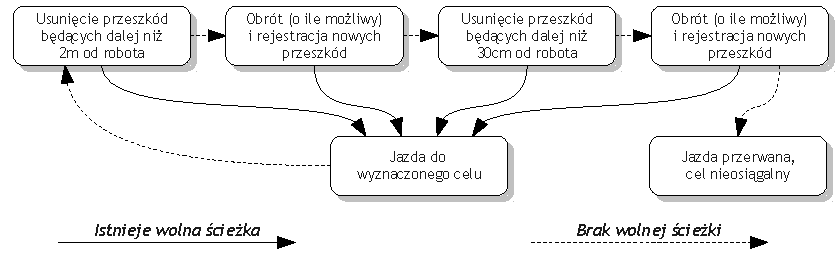
\includegraphics[width=\textwidth]{../img/recovery}
\caption{Zachowania ratunkowe}
\label{fig:recovery}
\end{figure}

\section{Weryfikacja poprawności działania}

Największym problemem w~aplikacjach robotycznych jest weryfikacja poprawności ich
działania. Możliwe jest napisanie testów jednostkowych samego oprogramowania,
nie da się jednak stworzyć podobnych testów dla aplikacji wykorzystujących sprzęt
taki jak roboty. Istnieje kilka podejść przeprowadzania testów mających na celu
zwiększenie prawdopodobieństwa działania aplikacji zgodnie z~oczekiwaniami.
Pierwszą metodą jest wykorzystanie symulatorów (zarówno ogólnodostępnych, jak
i~specjalizowanych przygotowywanych specjalnie dla jednego robota). Kolejnym sposobem
jest przetestowanie aplikacji z~wykorzystaniem właściwego robota w~kontrolowanych
warunkach (z zachowaniem odpowiednich środków ostrożności). Istotne jest to, że
obie te metody można wykorzystać jednocześnie, sprawdzając najpierw ogólną poprawność
algorytmu na symulacji, a~następnie sprawdzając wszystkie możliwe przypadki użycia
(a przynajmniej tyle, ile można przewidzieć).

\subsection{Wykorzystanie symulacji}

Obecnie istnieje wiele gotowych symulatorów do testowania zachowań robotów
mobilnych, występują zarówno w~wersjach dwuwymiarowych (Stage) jak i~trójwymiarowych
(Gazebo). Posiadają możliwość pełnej symulacji układu robotycznego, zarówno
jego bazy jezdnej jak i~wielu różnych sensorów. Dodatkowo wyposażone są 
w~moduł symulacji fizycznej, dzięki czemu symulacje mogą odwzorowywać dodatkowe
czynniki, takie jak różne współczynniki tarcia podłoża czy zderzenia. 
Niestety, wielu elementów nie da się dokładnie zasymulować, chociażby ze
względu na występujące niedokładności rzeczywistych czujników, często o~charakterze
losowym i~różnego rodzaju szumy. Poza tym w~warunkach symulacji zazwyczaj dużo
lepiej działają wszystkie systemy lokalizacji. 

Mimo opisanych cech symulacji, jest to najlepsze narzędzie do przeprowadzania
wstępnych testów algorytmów sterowania. Nie ma ryzyka uszkodzenia sprzętu
przy wystąpieniu dużego błędu, można też zgrubnie dobrać wstępne wartości
parametrów różnych algorytmów. Podczas prac z~robotem Elektron wykorzystywany
był symulator Gazebo, wraz z~trójwymiarowym modelem robota i~prostym modelem
środowiska zawierającym kilka przeszkód. Podczas tych kilku pierwszych uruchomień
ustalone zostały takie parametry wielkości map i~dokładności różnych algorytmów,
aby nie występowało nadmierne obciążenie procesora na komputerze sterującym
robota.

\subsection{Testy w~kontrolowanych warunkach}

Po dobraniu wstępnych wartości dla algorytmów (zarówno lokalizacji jak 
omijania przeszkód) rozpoczęły się testy na właściwym sprzęcie. Pierwsze 
przejazdy odbywały się ze zmniejszoną prędkością, w~środowisku pozbawionym
przeszkód i~miały na celu sprawdzenie w~rzeczywistości poprawności pracy
wszystkich elementów nawigacji.

Pierwsze testy dotyczyły działania systemu lokalnej i~globalnej lokalizacji.
Po skalibrowaniu żyroskopu i~odometrii robot został ustawiony w~znanym położeniu
(oznaczonym później na mapie jako miejsce startowe) i~był sterowany przy pomocy
joysticka i~modułu teleoperacji. Podczas ruchu wykonywane były różne trajektorie,
m.in. jazda po prostej, zakręty o~różnym promieniu i~prędkości pokonywania
oraz nagłe zmiany szybkości ruchu. Podczas całego testu system lokalizacji 
globalnej utrzymywał poprawne położenie robota w~odniesieniu do zgrubnej mapy 
pomieszczenia, czasami jedynie gubiąc się w~długim korytarzu pozbawionym 
cech charakterystycznych. System lokalizacji lokalnej po powrocie do punktu 
startowego wykazywał różnicę zarówno w~położeniu jak i~orientacji, wartości
te wahały się od kilkunastu centymetrów przy krótkich trasach do nieco ponad
metra przy długich testach (wartość różnicy w~orientacji wynosiła maksymalnie 10\textdegree,
dokładniejsze dane dotyczące dokładności systemu lokalizacji lokalnej podane
są w~części dotyczącej rozszerzonego filtru Kalmana).

Kolejnym testowanym modułem był globalny planer trasy. Testy polegały na 
wyznaczaniu robotowi różnych punktów docelowych, z~czego były możliwe 
trzy sytuacje: punkt osiągalny bez dodatkowych warunków, punkt osiągalny 
o~ile konfiguracja przeszkód na to pozwalała (w~tym przypadku zawsze pozwalała, 
miało to znaczenie przy kolejnych testach, gdzie pojawiły się przeszkody) 
oraz punkt nieosiągalny. W~każdym przypadku wykonano kilkanaście testów,
w~każdym przypadku trajektoria została wyznaczona prawidłowo i~robot wykonał
ją bez błędów, punkty docelowe nieosiągalne zostały wykryte i~odrzucone przez 
algorytm wyznaczania trajektorii. W~tych samych testach sprawdzana była także
poprawność wykonywania trajektorii przez moduły planera trajektorii lokalnej.
Po dostrojeniu odpowiednich parametrów (głównie dotyczących w~tym przypadku
czasu planowania wprzód tak, aby uniknąć jazdy w~kółko) robot przeszedł
testy bezbłędnie (za każdym razem trajektoria lokalna śledziła globalną 
bez kłopotów). 

Po przetestowaniu zdolności śledzenia zadanej ścieżki testy przeniosły się
na moduł wykrywania i~omijania przeszkód. W~tym momencie kluczowe były dwie
kwestie: dokładne skalibrowanie chmury punktów uzyskiwanej z~sensora Kinect
tak, aby punkty odpowiadające podłodze leżały na płaszczyźnie o~równaniu
$z=0$, oraz ustawienie odpowiednich wartości dla wielkości oczka siatki
w~lokalnej mapie zajętości. Pierwsze zadanie wykonywane jest przed rozpoczęciem
jazdy przez robota przy użyciu małej aplikacji, która pozycjonuje Kinect 
pod kątem 20\textdegree ~w dół, a~następnie odczytując dane z~wbudowanego 
w~niego akcelerometru wyznacza faktyczne wartości kątów pochylenia i~skręcenia
używane przy przekształcaniu chmury z~układu związanego z~czujnikiem do układu
związanego z~robotem. 

Dobór wielkości oczek lokalnej mapy zajętości miał kluczowe znaczenie przy zdolności
do pokonywania wąskich przejazdów przez robota. Przy zbyt dużej ich wielkości
przejazdy pomiędzy przeszkodami mogłyby stać się nieprzejezdne dla planera 
ścieżki lokalnej, przy zbyt małej robot mógł zacząć wpadać na niektóre przeszkody
podczas wykonywania obrotów w~ich pobliżu, wzrosłoby też znacząco obciążenie
systemu. Wartość była dobierana eksperymentalnie w~taki sposób, aby robot był
w~stanie przejechać przez drzwi o~szerokości 80cm, pod możliwie wieloma kątami
(a więc nie tylko na wprost). Oczka o~wielkości 10cm okazały się zdecydowanie 
zbyt mało dokładne, średnio w~70\% przypadków futryny po zaznaczeniu na mapie 
znajdowały się w~odległości 60cm, a~po uwzględnieniu dodatkowej (dość niskiej, 
bo jedynie 5cm) wartości dozwolonego dystansu od przeszkód okazywało się, że
robot nie jest w~stanie zmieścić się w~drzwiach (poprzez zmieszczenie się
rozumiana jest możliwość przejazdu przez drzwi oraz wykonania obrotu stojąc 
pomiędzy futrynami). Siatka wielkości 5cm dużo dokładniej pokrywała przeszkody,
pozwalając na przejazd robota przez wąskie przesmyki. Niestety, z~powodu dodatkowego 
obciążenia systemu konieczna stała się redukcja wielkości lokalnej mapy zajętości
z~początkowych dziewięciu do sześciu metrów (a więc po trzy metry od robota 
w~każdą stronę). 

Po kalibracji orientacji czujnika robot miał za zadanie pokonać trasy podobne,
jak przy poprzednich testach, tym razem mając na trasie ustawione dodatkowe
przeszkody (takie jak krzesła i~kartonowe pudełka). Planer trajektorii 
globalnej wyznaczał oczywiście ścieżki nie uwzględniające ich, gdyż nie 
były one zaznaczone na mapie, a~więc zadanie ich ominięcia spoczywało na
planerze lokalnym. Przy tym samym punkcie startowym i~docelowym oraz tej 
samej konfiguracji przeszkód robot wykonał po 10 przejazdów w~obie strony 
(od punktu startowego do docelowego i~z powrotem), z~czego w~dwóch przypadkach 
nastąpił kontakt z~przeszkodą. Kontakt polegał na zahaczeniu podczas zakręcania
o~najbardziej wystające elementy podstawy fotela biurowego i~jego delikatne 
przesunięcie, było to spowodowane małą wielkością oczka siatki w~mapie zajętości
i~dość wąskim polem widzenia sensora. Przeprowadzone zostały także testy 
wykrywania sytuacji wyjątkowych opisanych wcześniej. Robot podczas ruchu 
został otoczony przeszkodami (kartonowe pudła oraz ludzie) w~odległości 
ok. metra. Początkowo algorytm wyznaczał ścieżkę omijającą przeszkodę przed 
robotem, jednak wraz z~zakręcaniem wykrywane były kolejne, aż w~końcu wokół
całego robota na mapie zajętości pojawiły się przeszkody. W~tym momencie 
robot się zatrzymał i~rozpoczął wykonywanie zachowań ratunkowych. Jeśli 
w~tym czasie przeszkody zostały usunięte, robot kontynuował jazdę do celu,
jeśli natomiast pozostały na swoim miejscu, to po wykonaniu całej serii 
wszystkich przewidzianych ruchów i~aktualizacji mapy zajętości robot sygnalizował
prawidłowo niemożność osiągnięcia celu. 

Podczas testów z~przeszkodami zostało też sprawdzone wykrywanie nieprzejezdnych
obszarów (np. zamkniętych drzwi). Jeśli robot miał za zadanie przejechać pomiędzy
dwoma pomieszczeniami, gdzie przejazd możliwy był tylko przez jedne drzwi,
a~podczas przejazdu dojechał do zamkniętych drzwi, zatrzymywał się. W~tym 
momencie uruchamiany był ponownie globalny planer trasy, który oczywiście
nie był w~stanie jej znaleźć i~sygnalizowany był błąd (punkt docelowy jest
nieosiągalny). Podobna sytuacja (zatrzymanie robota i~ponowne generowanie 
ścieżki globalnej) występowała też podczas normalnego ruchu, kiedy istniało
kilka możliwych (z punktu widzenia dostarczonej mapy) dróg, a~wybrana okazywała
się nieprzejezdna (np. prowadziła przez obszar zastawiony krzesłami). W~tym 
wypadku po ponownym wyliczeniu robot kontynuował jazdę inną trasą.

\section{Eksperymenty porównawcze}

Po przeprowadzeniu niezbędnych testów (zarówno w~symulacji jak i~na rzeczywistym
sprzęcie) nadszedł czas na przeprowadzenie właściwych eksperymentów mających
na celu stwierdzenie czy i~w jaki sposób wykorzystanie kamery 3D wpływa na
proces nawigacji robota mobilnego. Podstawowym czujnikiem, z~którym porównywany
był Kinect był skaner laserowy Sick. Przygotowane zostały dwie trasy, zawierające
różne rodzaje przeszkód. Pierwsza zawierająca jedynie kartonowe pudła oraz
stoły (pod którymi robot mógł bezpiecznie przejechać, przeszkodę stanowiły 
jedynie ich nogi), druga składająca się dodatkowo z~krzeseł biurowych oraz
małych niskich pudełek (ok. 10cm wysokości). 

W pierwszym przypadku zarówno skaner laserowy jak i~Kinect wykrywały przeszkody 
w~ten sam sposób (niezależnie od wysokości przeszkody miały ten sam kształt), 
więc nie było widać przewagi kamery 3D nad klasycznym laserem. Dodatkowo z~powodu
wąskiego pola widzenia sensora 3D podczas wykonywania trajektorii robot częściej
musiał się obracać aby zbadać obszar po bokach, pomiary z~lasera od razu
pokazywały prawie całe otoczenie, więc trajektorie były gładsze i~ogólna
szybkość ich pokonywania była większa o~ok. 30\% .

W drugim wypadku wykorzystanie sensora 3D dało wymierne rezultaty -- wykrywał
on bezbłędnie wszystkie przeszkody, w~tym niskie pudełka (całkowicie niewidoczne
przy pomiarach laserowych) oraz podstawy krzeseł biurowych (w~tym przypadku 
na skanerze laserowym widoczne były jedynie ich wąskie nogi). W~wielu wypadkach
skutkowało to wpadaniem na te przeszkody przy korzystaniu ze skanera laserowego
(praktycznie w~każdym przejeździe robot wpadał na małe pudełka, co jest 
oczywiste biorąc pod uwagę że całkowicie nie był w~stanie ich wykryć, dodatkowo
w~ok. połowie przypadków zahaczał o~podstawy krzeseł biurowych próbując 
przejechać w~ich pobliżu). Taki scenariusz rozmieszczenia przeszkód jest 
dużo bardziej realistyczny w~warunkach normalnej eksploatacji pomieszczeń 
biurowych i~podobnych, widać więc zdecydowaną zaletę z~korzystania z~czujników
zwracających pełny, trójwymiarowy obraz sceny przed robotem. 

W ramach ostatniego testu do nawigacji zostały wykorzystane oba dostępne czujniki 
-- zarówno skaner laserowy jak i~sensor Kinect. W~tym wypadku rezultaty były 
najlepsze ze wszystkich -- wykrywane były wszystkie przeszkody przed robotem
(nawet najmniejsze i~o nieregularnym kształcie), a~dzięki zastosowaniu skanera
o~dużym polu widzenia część przeszkód po bokach także była zaznaczana powodując,
że planer ścieżki lokalnej nie musiał wykonywać dodatkowych obrotów w~celu 
zbadania przejezdności tych obszarów.
